% 柱坐标系

\pentry{极坐标系\upref{Polar}}
若在原有的直角坐标系上定义柱坐标系(\autoref{Cylin_fig1}),可用三个变量 $(r, \theta, z)$ 描述三维空间中任意一点.其中 $r$ 代表该点到 $z$ 轴的距离( $r \ges 0$), $\theta$ 代表与 $x$ 轴的夹角,$z$ 与直角坐标系相同. 柱坐标系相当于在极坐标系的基础上增加了一个垂直轴.

\begin{figure}[ht]
\centering
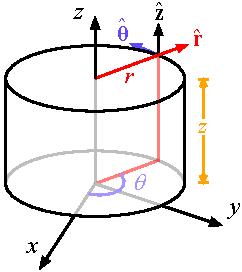
\includegraphics[width=4.5cm]{./figures/Cylin1.pdf}
\caption{定义柱坐标系}\label{Cylin_fig1}
\end{figure}

柱坐标系中的单位矢量如\autoref{Cylin_fig1} 中的 $\uvec r,\uvec \theta ,\uvec z$ 所示. 其中 $\uvec r, \uvec \theta$ 与极坐标系中的定义相同, $\uvec z$ 是直角坐标系 $z$ 轴的单位矢量, 注意三个单位矢量两两垂直, 构成一组单位正交基底, 任何矢量可以在这组基底上展开. 再次强调, 与直角坐标系不同的是, $\uvec r, \uvec \theta$ 并不是常矢量, 而是坐标 $\theta$ 的函数.

柱坐标与直角坐标间的转换类比\autoref{Polar_eq2}\upref{Polar} 和\autoref{Polar_eq4}\upref{Polar} 即可
\begin{equation}
\leftgroup{x &= r\cos \theta \\
y &= r\sin \theta \\
z &= z}
\qquad
\leftgroup{r &= \sqrt {x^2 + y^2} \\
\theta  &= \Arctan(y, x)\\
z &= z}
\end{equation}

















